\lecture{10}{6 Nov.}{}

The computation at the end of \autoref{sec:covering} shows where a one-shot random choice loses. With \(p = \frac{t}{D}\), a fixed \(\ell\)-set lies in \(t\) chosen \(k\)-sets on average. If \(t\) is large, many \(\ell\)-sets are covered several times and the extra \(k\)-sets are wasted; if \(t\) is small, a fraction \(e^{-t}\) of the \(\ell\)-sets stays uncovered; no constant \(t\) avoids both losses. R\"odl's way out is to choose only a small random batch of \(k\)-sets at a time, a \emph{nibble}, discard the \(\ell\)-sets it covers, and repeat on what is left. Only the incidences between \(\ell\)-sets and \(k\)-sets matter for this, so we first restate the problem as covering the vertices of a hypergraph.

\section{Covers in Hypergraphs}\label{sec:hypergraph-covers}

A \vocab{cover} of a hypergraph \(H\) is a set of edges whose union is \(V(H)\).

\begin{definition}[Auxiliary hypergraph]\label{def:aux-hypergraph}
    For \(n \ge k \ge \ell \ge 1\), let \(\mathcal{H}\) be the hypergraph with
    \[
        V(\mathcal{H}) = \binom{[n]}{\ell},
        \qquad
        E(\mathcal{H}) = \Bigl\{ e_K : K \in \binom{[n]}{k} \Bigr\},
        \quad\text{where } e_K \coloneqq \binom{K}{\ell}.
    \]
    So the vertices are the \(\ell\)-sets, and the edge \(e_K\) is the set of \(\ell\)-sets covered by the \(k\)-set \(K\); \(\mathcal{H}\) is \(\binom{k}{\ell}\)-uniform.
\end{definition}

An \(\ell\)-set \(X\) lies in \(e_K\) iff \(X \subseteq K\). Hence \(S_1, \ldots, S_m\) cover every \(\ell\)-set iff \(e_{S_1}, \ldots, e_{S_m}\) cover \(V(\mathcal{H})\):
\[
    \text{covering \(\ell\)-subsets with \(k\)-subsets} \iff \text{covering \(V(\mathcal{H})\) with edges},
\]
and \(M(n,k,\ell)\) is the minimum size of a cover of \(\mathcal{H}\).

\begin{question}\label{q:hypergraph-cover}
    Given an \(r\)-uniform hypergraph on \(N\) vertices, how many edges do we need to cover all the vertices?
\end{question}

\emph{Trivial lower bound.} \(m\) edges of size \(r\) contain at most \(mr\) vertices, so a cover needs \(m \ge \frac{N}{r}\). For \(\mathcal{H}\) this is \(\frac{N}{r} = \binom{n}{\ell} \big/ \binom{k}{\ell}\), i.e.\ \autoref{prop:covering-lower}, and \autoref{thm:rodl} says that \(\mathcal{H}\) has a cover only a factor \(1 + o(1)\) above the trivial bound. In general the trivial bound can be off by a constant factor.

\begin{eg}\label{eg:cover-bad}
    Three \(3\)-uniform hypergraphs (\(r = 3\)) that need many more than \(\frac{N}{3}\) edges.
    \begin{center}
        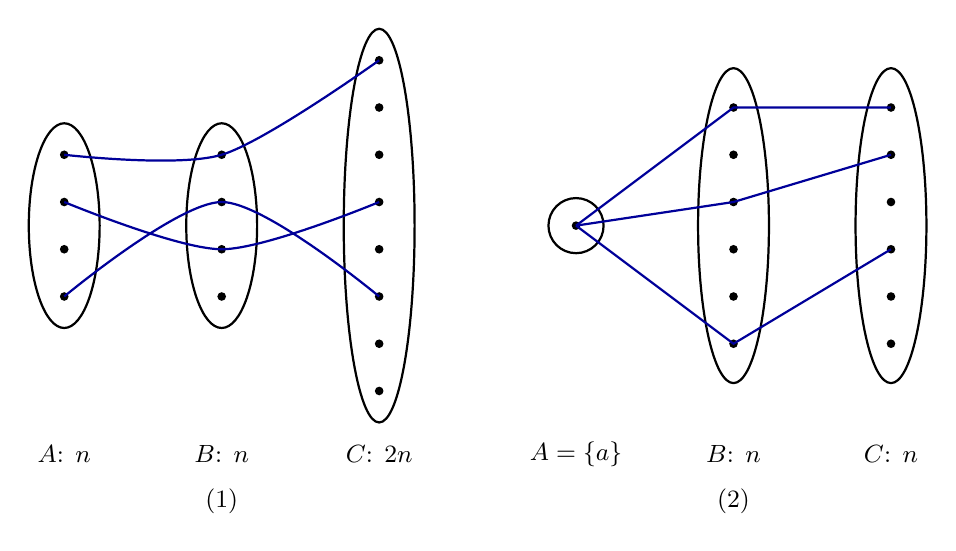
\begin{tikzpicture}[thick, every node/.style={font=\small}, dot/.style={circle, fill, inner sep=1.1pt}]
            \begin{scope}
                \draw (0,0) ellipse (0.45 and 1.3);
                \draw (2,0) ellipse (0.45 and 1.3);
                \draw (4,0) ellipse (0.45 and 2.5);
                \foreach \y in {0.9,0.3,-0.3,-0.9} {
                    \node[dot] at (0,\y) {};
                    \node[dot] at (2,\y) {};
                }
                \foreach \y in {2.1,1.5,0.9,0.3,-0.3,-0.9,-1.5,-2.1} \node[dot] at (4,\y) {};
                \draw[blue!60!black] plot[smooth] coordinates {(0,0.9) (2,0.9) (4,2.1)};
                \draw[blue!60!black] plot[smooth] coordinates {(0,0.3) (2,-0.3) (4,0.3)};
                \draw[blue!60!black] plot[smooth] coordinates {(0,-0.9) (2,0.3) (4,-0.9)};
                \node at (0,-2.9) {\(A\): \(n\)};
                \node at (2,-2.9) {\(B\): \(n\)};
                \node at (4,-2.9) {\(C\): \(2n\)};
                \node at (2,-3.5) {(1)};
            \end{scope}
            \begin{scope}[xshift=6.5cm]
                \draw (0,0) circle (0.35);
                \node[dot] (a) at (0,0) {};
                \draw (2,0) ellipse (0.45 and 2);
                \draw (4,0) ellipse (0.45 and 2);
                \foreach \y in {1.5,0.9,0.3,-0.3,-0.9,-1.5} {
                    \node[dot] at (2,\y) {};
                    \node[dot] at (4,\y) {};
                }
                \draw[blue!60!black] (0,0) -- (2,1.5) -- (4,1.5);
                \draw[blue!60!black] (0,0) -- (2,0.3) -- (4,0.9);
                \draw[blue!60!black] (0,0) -- (2,-1.5) -- (4,-0.3);
                \node at (0,-2.9) {\(A = \{a\}\)};
                \node at (2,-2.9) {\(B\): \(n\)};
                \node at (4,-2.9) {\(C\): \(n\)};
                \node at (2,-3.5) {(2)};
            \end{scope}
        \end{tikzpicture}
    \end{center}
    \begin{enumerate}[(1)]
        \item \(V = A \cupdot B \cupdot C\) with \(\abs{A} = \abs{B} = n\) and \(\abs{C} = 2n\), and every edge has one vertex in each part. Here \(N = 4n\) and \(\frac{N}{r} = \frac{4n}{3}\), but each edge contains only one vertex of \(C\), so a cover needs \(\ge 2n\) edges to cover \(C\).
        \item \(V = \{a\} \cupdot B \cupdot C\) with \(\abs{B} = \abs{C} = n\), and every edge is \(\{a, b, c\}\) with \(b \in B\), \(c \in C\). Here \(N = 2n + 1\) and \(\frac{N}{r} = \frac{2n+1}{3} \approx \frac{2}{3}n\), but again each edge contains one vertex of \(C\), so a cover needs \(\ge n\) edges.
        \item \(V\) is split into \(\frac{N}{9}\) disjoint \emph{layers} of \(9\) vertices, and no edge meets two layers. A layer consists of two triangles \(T\), \(T'\) (\(3\) vertices each) and three further vertices \(Z\), and its edges are the \(18\) sets \(\{u, v, z\}\) with \(uv\) one of the \(6\) sides of \(T\) or \(T'\) and \(z \in Z\).
        \begin{center}
            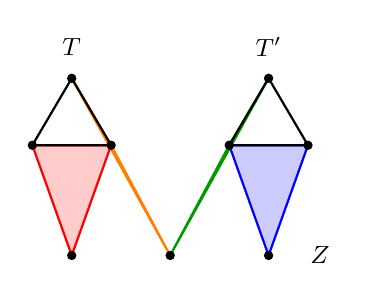
\begin{tikzpicture}[thick, every node/.style={font=\small}, dot/.style={circle, fill, inner sep=1.2pt}]
                \coordinate (x1) at (0,0); \coordinate (x2) at (1,0); \coordinate (x3) at (0.5,0.85);
                \coordinate (y1) at (2.5,0); \coordinate (y2) at (3.5,0); \coordinate (y3) at (3,0.85);
                \coordinate (z1) at (0.5,-1.4); \coordinate (z2) at (1.75,-1.4); \coordinate (z3) at (3,-1.4);
                \fill[red, opacity=0.2] (x1) -- (x2) -- (z1) -- cycle;
                \draw[red] (x1) -- (x2) -- (z1) -- cycle;
                \fill[orange, opacity=0.2] (x2) -- (x3) -- (z2) -- cycle;
                \draw[orange] (x2) -- (x3) -- (z2) -- cycle;
                \fill[blue, opacity=0.2] (y1) -- (y2) -- (z3) -- cycle;
                \draw[blue] (y1) -- (y2) -- (z3) -- cycle;
                \fill[green!60!black, opacity=0.2] (y1) -- (y3) -- (z2) -- cycle;
                \draw[green!60!black] (y1) -- (y3) -- (z2) -- cycle;
                \draw (x1) -- (x2) -- (x3) -- cycle;
                \draw (y1) -- (y2) -- (y3) -- cycle;
                \foreach \p in {x1,x2,x3,y1,y2,y3,z1,z2,z3} \node[dot] at (\p) {};
                \node at (0.5,1.25) {\(T\)};
                \node at (3,1.25) {\(T'\)};
                \node[right] at (3.4,-1.4) {\(Z\)};
            \end{tikzpicture}
        \end{center}
        A vertex of \(T\) lies on \(2\) sides and each side is in \(3\) edges, so it has degree \(2 \cdot 3 = 6\); a vertex of \(Z\) is in one edge per side, so it has degree \(6\). Thus this hypergraph is \(6\)-regular. Every edge meets \(T\) in \(0\) or \(2\) vertices and \(\abs{T} = 3\) is odd, so at least \(2\) edges meet \(T\); likewise for \(T'\), and no edge meets both. So each layer needs \(\ge 4\) edges (the picture shows a cover of a layer by \(4\)), and a cover needs \(\ge 4 \cdot \frac{N}{9} = \frac{4}{3} \cdot \frac{N}{3}\) edges in total.
    \end{enumerate}
\end{eg}

In (1) and (2) of \autoref{eg:cover-bad} the degrees are very uneven: in (1), every edge meets \(A\) and \(C\) once each, so
\[
    \sum_{x \in A} \deg(x) = \sum_{x \in C} \deg(x) = e(H)
    \qquad\text{while}\qquad
    \abs{C} = 2\abs{A},
\]
so a vertex of \(C\) has on average half the degree of a vertex of \(A\); and in (2), \(a\) lies in every edge. Example (3) is regular, but the two ends of a side of \(T\) lie together in \(3\) of the \(6\) edges at either of them, so the edges at a vertex keep reusing the same few other vertices. The next definition rules out both problems.

\begin{definition}[Degree, codegree]\label{def:codegree}
    Let \(H\) be a hypergraph and \(x, y \in V(H)\). The \vocab{degree} of \(x\) and the \vocab{codegree} of \(x\) and \(y\) are
    \[
        \deg(x) \coloneqq \#\{ e \in E(H) : x \in e \},
        \qquad
        \operatorname{codeg}(x,y) \coloneqq \#\{ e \in E(H) : x, y \in e \}.
    \]
\end{definition}

\begin{notation}
    \(a = (1 \pm \gamma) D\) means \((1 - \gamma) D \le a \le (1 + \gamma) D\).
\end{notation}

\begin{definition}[Well-spread]\label{def:well-spread}
    An \(r\)-uniform hypergraph \(H\) on \(N\) vertices is \vocab{\((\gamma, K)\)-well-spread} if there is a \(D\), the \vocab{typical degree}, such that
    \begin{enumerate}[(i)]
        \item for all but at most \(\gamma N\) vertices \(x\), \(\deg(x) = (1 \pm \gamma) D\);
        \item for all vertices \(x\), \(\deg(x) < K D\);
        \item for any two distinct vertices \(x, y\), \(\operatorname{codeg}(x,y) < \gamma D\).
    \end{enumerate}
\end{definition}

\begin{theorem}[Pippenger]\label{thm:pippenger}
    For every \(r \ge 2\), \(K \ge 1\) and \(a > 0\), there are \(\gamma = \gamma(r,K,a) > 0\) and \(D_0 = D_0(r,K,a)\) such that for every \(N\) and every \(D \ge D_0\) the following holds. If \(H\) is a \((\gamma, K)\)-well-spread \(r\)-uniform hypergraph on \(N\) vertices with typical degree \(D\), in which every vertex has positive degree,\footnote{A vertex of degree \(0\) lies in no edge and can never be covered, and (i) of \autoref{def:well-spread} allows up to \(\gamma N\) such vertices.} then \(H\) has a cover of size at most \((1 + a) \frac{N}{r}\).
\end{theorem}

\begin{observation}
    \autoref{thm:pippenger} implies \autoref{thm:rodl}.
\end{observation}

\begin{proof}
    If \(k = \ell\), every \(\ell\)-set needs its own \(k\)-set, so \(M(n,k,\ell) = \binom{n}{\ell} = \binom{n}{\ell} \big/ \binom{k}{\ell}\). Let \(k > \ell\), and apply \autoref{thm:pippenger} to \(\mathcal{H}\) from \autoref{def:aux-hypergraph}, which has
    \[
        N = \binom{n}{\ell},
        \qquad
        r = \binom{k}{\ell},
        \qquad
        D \coloneqq \binom{n-\ell}{k-\ell}.
    \]
    \begin{itemize}
        \item \emph{Degrees.} A \(k\)-set \(K \supseteq X\) is \(X\) together with a \((k-\ell)\)-subset of \([n] \setminus X\), so \(\deg(X) = \binom{n-\ell}{k-\ell} = D\) for every vertex \(X\). Hence (i) holds for every \(\gamma\), (ii) holds with \(K = 2\), and every degree is positive.
        \item \emph{Codegrees.} Let \(X \ne Y\) and pick \(y \in Y \setminus X\). Every \(k\)-set containing \(X\) and \(Y\) contains the \((\ell+1)\)-set \(X \cup \{y\}\), so, using \(\binom{m-1}{j-1} = \frac{j}{m}\binom{m}{j}\) with \(m = n - \ell\), \(j = k - \ell\),
        \[
            \operatorname{codeg}(X,Y) \le \binom{n-\ell-1}{k-\ell-1} = \frac{k-\ell}{n-\ell} \binom{n-\ell}{k-\ell} = \frac{k-\ell}{n-\ell}\, D = o(D).
        \]
    \end{itemize}
    Fix \(a > 0\) and let \(\gamma = \gamma(r,2,a)\), \(D_0 = D_0(r,2,a)\). For \(n\) large, \(\frac{k-\ell}{n-\ell} < \gamma\), so (iii) holds, and \(D \ge n - \ell \ge D_0\). \autoref{thm:pippenger} gives a cover of \(\mathcal{H}\) of size \(\le (1+a)\frac{N}{r}\), and with \autoref{prop:covering-lower},
    \[
        \frac{\binom{n}{\ell}}{\binom{k}{\ell}} \le M(n,k,\ell) \le (1 + a) \frac{\binom{n}{\ell}}{\binom{k}{\ell}}
        \qquad\text{for all large } n .
    \]
    As \(a > 0\) is arbitrary, \(M(n,k,\ell) = (1 + o(1)) \binom{n}{\ell} \big/ \binom{k}{\ell}\).
\end{proof}

\section{Taking a Nibble}\label{sec:nibble}

Let \(H\) be well-spread with typical degree \(D\). What if we take \(m\) edges uniformly and independently at random? Pretend every degree is \(D\); then \(\sum_{x} \deg(x) = r\, e(H)\) gives \(e(H) \approx \frac{ND}{r}\). Each random edge contains \(v\) with probability \(\frac{\deg(v)}{e(H)}\), so
\[
    \mathbb{P}(v \text{ is uncovered}) = \Bigl( 1 - \frac{\deg(v)}{e(H)} \Bigr)^{m} \approx \Bigl( 1 - \frac{D}{ND/r} \Bigr)^{m} = \Bigl( 1 - \frac{r}{N} \Bigr)^{m} \approx e^{-\frac{rm}{N}},
\]
where \(\frac{rm}{N} \approx m \cdot \frac{\deg(v)}{e(H)}\) is the expected number of times \(v\) is covered.
\begin{center}
    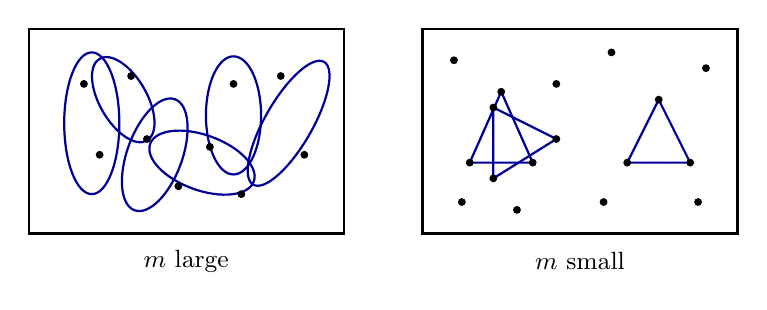
\begin{tikzpicture}[thick, every node/.style={font=\small}, dot/.style={circle, fill, inner sep=1pt}]
        \draw (0,0) rectangle (4,2.6);
        \draw[blue!60!black] (0.8,1.4) ellipse (0.35 and 0.9);
        \draw[blue!60!black, rotate around={30:(1.2,1.7)}] (1.2,1.7) ellipse (0.3 and 0.6);
        \draw[blue!60!black, rotate around={-20:(1.6,1)}] (1.6,1) ellipse (0.35 and 0.75);
        \draw[blue!60!black, rotate around={70:(2.2,0.9)}] (2.2,0.9) ellipse (0.35 and 0.7);
        \draw[blue!60!black] (2.6,1.5) ellipse (0.35 and 0.75);
        \draw[blue!60!black, rotate around={-30:(3.3,1.4)}] (3.3,1.4) ellipse (0.3 and 0.9);
        \foreach \p in {(0.7,1.9),(0.9,1),(1.3,2),(1.5,1.2),(1.9,0.6),(2.3,1.1),(2.6,1.9),(2.7,0.5),(3.2,2),(3.5,1)} \node[dot] at \p {};
        \node at (2,-0.35) {\(m\) large};
        \begin{scope}[xshift=5cm]
            \draw (0,0) rectangle (4,2.6);
            \foreach \p in {(0.4,2.2),(0.5,0.4),(1.2,0.3),(2.4,2.3),(3.6,2.1),(3.5,0.4),(2.3,0.4),(1.7,1.9)} \node[dot] at \p {};
            \draw[blue!60!black] (0.6,0.9) -- (1.4,0.9) -- (1,1.8) -- cycle;
            \draw[blue!60!black] (0.9,0.7) -- (1.7,1.2) -- (0.9,1.6) -- cycle;
            \draw[blue!60!black] (2.6,0.9) -- (3.4,0.9) -- (3,1.7) -- cycle;
            \foreach \p in {(0.6,0.9),(1.4,0.9),(1,1.8),(0.9,0.7),(1.7,1.2),(0.9,1.6),(2.6,0.9),(3.4,0.9),(3,1.7)} \node[dot] at \p {};
            \node at (2,-0.35) {\(m\) small};
        \end{scope}
    \end{tikzpicture}
\end{center}
The two pictures are the trade-off from the start of the lecture. If \(\frac{rm}{N}\) is large, almost every vertex is covered but many are covered several times. If \(m = \frac{\varepsilon N}{r}\) for a small \(\varepsilon\), each vertex is covered with probability \(\approx 1 - e^{-\varepsilon} \approx \varepsilon\) and overlaps are rare: the nibble covers about \(\varepsilon N - O(\varepsilon^{2} N)\) of the \(\varepsilon N\) vertices it could cover at best. So we take a nibble, delete the covered vertices and repeat. This only works if what remains is again well-spread, which is what the key lemma provides.

\begin{lemma}[Key lemma]\label{lem:nibble}
    For every \(r \ge 2\), \(K \ge 1\), \(\varepsilon > 0\) and \(\delta' > 0\), there are \(\delta = \delta(r,K,\varepsilon,\delta') > 0\) and \(D_0 = D_0(r,K,\varepsilon,\delta')\) such that for every \(N\) and every \(D \ge D_0\) the following holds. If \(H\) is a \((\delta, K)\)-well-spread \(r\)-uniform hypergraph on \(N\) vertices with typical degree \(D\), then there is a set \(E'\) of edges with
    \begin{enumerate}[(i)]
        \item \(\abs{E'} = \frac{\varepsilon N}{r} (1 \pm \delta')\);
        \item the set \(V' \coloneqq V \setminus \bigcup_{e \in E'} e\) of uncovered vertices has \(\abs{V'} = N e^{-\varepsilon} (1 \pm \delta')\);
        \item all but at most \(\delta' \abs{V'}\) vertices of \(V'\) have degree \(D e^{-\varepsilon(r-1)} (1 \pm \delta')\) in the induced hypergraph \(H[V']\).
    \end{enumerate}
\end{lemma}

The numbers in \autoref{lem:nibble} match the heuristic above with \(m = \frac{\varepsilon N}{r}\). (ii) is \(\mathbb{P}(v \text{ uncovered}) \approx e^{-\varepsilon}\). For (iii), an edge \(e \ni x\) with \(x \in V'\) survives in \(H[V']\) iff its other \(r - 1\) vertices are also uncovered, which happens with probability \(\approx (e^{-\varepsilon})^{r-1}\). Thus \(H[V']\) is again nearly regular, with about \(N e^{-\varepsilon}\) vertices and typical degree about \(D e^{-\varepsilon(r-1)}\), so the lemma can be applied to it again.
